This chapter evaluates the outcomes of the project by analyzing the responses generated by LLaMa model following prompt engineering modifications. The evaluation focuses on several key aspects: the accuracy, coherence, relevance, and adaptability of the responses to incremental prompts scenarios, by adding at each iteration the strategies discussed in the previous chapters. In a qualitative assessment perspective, the analysis aims to highlight the improvements achieved through prompt engineering and identify areas for further enhancement. This comprehensive evaluation not only underscores the efficacy of the applied strategies but also provides insights into the model's performance across different dimensions of language understanding and generation. The subsequent sections present the outcomes across four distinct configurations: a baseline environment with no modifications, after the implementation of role prompting, following the addition of a RAG approach, and ultimately, after incorporating an agentic behaviour.




\section{Conversations and the main observations}
\label{sec:conversations}


\subsection{Baseline environment}
\label{sec:baseline}

The instruction-tuned language model facilitates a simple yet effective interaction, enabling a natural conversational flow: the conversation holds meaning in a general purpose interaction.

\begin{Verbatim}[breaklines=true]
\underline{USER}:       Hey, can you tell me any fun attraction to visit?

\underline{ASSISTANT}:  There are countless amazing attractions around the world, but I'll give you some popular and unique ones to consider:

1. The Great Barrier Reef (Australia): As the world's largest coral reef system, it's a snorkeler's and scuba diver's paradise.
2. The Grand Canyon (USA): One of the most iconic natural wonders in the United States, offering breathtaking views and hiking opportunities.
3. The Great Wall of China (China): A series of fortifications built to protect the Chinese Empire, now a UNESCO World Heritage Site.
4. The Eiffel Tower (France): An iconic symbol of Paris, offering stunning views of the city from its top.
5. The Taj Mahal (India): A beautiful white marble mausoleum built by the Mughal Empire, a testament to love and beauty.
6. The Colosseum (Italy): An ancient amphitheater in the heart of Rome, a symbol of the Roman Empire's engineering and architectural prowess.
7. The Aurora borealis (Northern Lights) (Arctic Circle): A natural light display that's a sight to behold.
8. The Golden Gate Bridge (USA): An iconic suspension bridge in San Francisco, offering stunning views of the Bay Area.
9. The Pyramids of Giza (Egypt): The last remaining ancient wonder of the Seven Wonders of the Ancient World, a must-visit for history buffs.
10. The Christ the Redeemer statue (Brazil): A massive Art Deco statue of Jesus Christ in Rio de Janeiro, offering breathtaking views of the city.

Some unique attractions to consider:

1. The Hang Son Doong cave (Vietnam): The world's largest cave, with its own jungle, river, and even its own climate.
2. The Trolltunga rock formation (Norway): A challenging hike rewarded with a unique rock formation resembling a troll's tongue.
3. The Glowworm Grotto (New Zealand): A cave filled with thousands of glowworms, creating a magical atmosphere.
4. The Chocolate Hills (Philippines): A unique geological formation of over 1,000 conical hills, perfect for hiking and exploration.
5. The Salar de Uyuni (Bolivia): The world's largest salt flat, creating a surreal landscape of white salt and mirror-like reflections.

\underline{USER}:       What do you suggest seeing in 24 hours in Verona, Italy?

\underline{ASSISTANT}:  Verona, the City of Love! With only 24 hours, you can still experience the best of Verona's romantic atmosphere, rich history, and stunning architecture. Here's a suggested itinerary to make the most of your time:

Morning (9:00 AM - 12:00 PM)

1. Piazza delle Erbe: Start your day in the heart of Verona's historic center, surrounded by beautiful buildings, cafes, and shops. Admire the stunning architecture, and take a photo in front of the Aquila Fountain.
2. Ponte Pietra: Walk across this ancient Roman bridge, offering breathtaking views of the Adige River and the city.
3. Verona Cathedral (Duomo): Visit the stunning cathedral, a masterpiece of Romanesque architecture, and climb to the top for panoramic views of the city.

Lunchtime (12:00 PM - 1:30 PM)

1. Try some local cuisine: Enjoy a traditional Veronese lunch at a local trattoria, such as La Grotta or Trattoria al Pompiere. Be sure to try the famous Risotto alla Pilota and Prosciutto di Verona.

Afternoon (1:30 PM - 5:00 PM)

1. Juliet's Balcony: Visit the famous balcony where Juliet Capulet is said to have stood in Shakespeare's Romeo and Juliet. Take a photo in front of the balcony, and explore the adjacent Casa di Giulietta (Juliet's House).
2. Piazza dei Signori: Explore this charming square, surrounded by beautiful buildings, and visit the Torre dei Lamberti, a 12th-century tower offering stunning views of the city.
3. Verona Arena: Visit this ancient Roman amphitheater, one of the best-preserved in the world, and imagine the gladiators who once fought here.

Evening (5:00 PM - 8:00 PM)

1. Admire the sunset: Find a spot with a view, such as the Ponte Pietra or the Torre dei Lamberti, to watch the sunset over the city.
2. Dinner: Enjoy a romantic dinner at a local restaurant, such as La Taverna del Leone or Ristorante La Fontanella.
\end{Verbatim}

As can be noted, the model succeeds in returning meaningful interactions, gathering the knowledge acquired in the training phase and responding accordingly. Lacking of a give context, to the query \textit{Hey, can you tell me any fun attraction to visit?}, the assistant takes the whole world as its competence, citing the Great Barrier Reef, the Eiffel Tower and the Taj Mahal. However, as soon as we restrain the focus querying \textit{What do you suggest seeing in 24 hours in Verona, Italy?}, the expertise on the city of Verona becomes aware, thus returning the most famous points of interest--and, in this case, also a plan for visiting the city. It is dutiful though that an assistant must be readily aware of the domain involved in the conversation, and this behaviour is enhanced as soon as a context is introduced.


\subsection{Being a Tour Guide}
\label{sec:tour-guide}

In a first attempt of interacting with the chatbot, it was evident that a context awareness was lacking, but as some information is injected into the model's context, a specific behaviour is triggered, accessing a restricted punctual knowledge that was already part of the baseline repository. In particular, the System prompt havs been introduced, in order to set both the context and the role, as seen in Section \ref{sec:prompt-anatomy}:

\begin{Verbatim}[breaklines=true]
You are a tour guide assisting tourists in Verona, Italy. Your job is to suggest users with new attractions to visit, based on the previous attractions visited and users' preferences. Tourists have a pass named Veronacard, for which they have access to all points of interests in the city, for 24, 48 or 72 hours. Your tone is both professional and friendly at the same time.
\end{Verbatim}

This snippet sets a touristic context, and the role that the model must adopt is an assisting guide. Citing the VeronaCard, further restricts the set of target user, making the response fully engaged:

\begin{Verbatim}[breaklines=true]
\underline{SYSTEM}:     You are a tour guide assisting tourists in Verona, Italy. Your job is to suggest users with new attractions to visit, based on the previous attractions visited and users' preferences. Tourists have a pass named Veronacard, for which they have access to all points of interests in the city, for 24, 48 or 72 hours. Your tone is both professional and friendly at the same time.

\underline{USER}:       Hey, can you tell me any fun attraction to visit?

\underline{ASSISTANT}:  Of course! There are so many things to see in Verona, I would begin with visiting the famous Arena.

\underline{USER}:       What do you suggest seeing in 24 hours?

\underline{ASSISTANT}:  With your 24-hour Veronacard, you can definitely see the main attractions. 

First, start your day at the Arena di Verona, the ancient Roman amphitheater that hosts the famous Opera Festival every summer. Then, take a stroll through the Piazza Bra, the largest square in Verona, and visit the nearby Museo di Castelvecchio, a stunning 14th-century castle that now houses a museum with an impressive collection of art and artifacts.

Next, take a romantic gondola ride along the Adige River and pass under the famous Ponte Pietra, a beautiful Roman bridge. After that, visit the Casa di Giulietta (Juliet's House), a 14th-century house that inspired Shakespeare's famous balcony scene from Romeo and Juliet.

Finally, end your day with a visit to the Torre dei Lamberti, a 12th-century tower that offers breathtaking views of the city. With the Veronacard, you can skip the lines and enjoy all these attractions without any hassle.
\end{Verbatim}

Using the same initial user prompt as the baseline case (i.e., \textit{Hey, can you tell me any fun attraction to visit?}) the response is coherent to the task, that is, suggesting the Arena di Verona in the first place. Note: the answer given here is intentionally shorter having set a smaller token output limit, because whenever a limit is not set, the model can take as much freedom in the quantity of tokens generated.

Then, it can be noticed that give the input \textit{What do you suggest seein in 24 hours?}, the corresponding answer is similar to the baseline case, highlighting a plan of todos throughout the day: the behaviour is similar but not equal, as the specification \textit{Your tone mis both professional and friendly at the same time.}, here \textit{friendly} may have changed the format of the roadmap suggested.

Overall, the model demonstrated the capacity to maintain a professional yet friendly conversational tone, effectively emulating the role of a knowledgeable local tour guide. This approach not only enriches the user's engagement but also ensures that responses are concise, relevant, and practically beneficial.


\subsection{Points of Interest and Weather}
\label{sec:pois-weather}

In the previous section setting a context aided the model to give more concise responses, readily able to suggest things to do in Verona, although not explicitly mentioned by the incoming query. Now, the next step involves further convey the possible set of responses to the specific tasks desired: which points of interest to address and weather data integration. The first piece of information is easily retrieved from the VeronaCard dataset as stated in Section \ref{sec:veronacard}: whereas the native knowledge of Verona is larger than the one required by the project, potentially recommending many more activities, the domain was restricted in order to be linked with the affluency data (which will be discussed in the next section). The weather data is fetched and prepared beforehand through the API seen in Section \ref{sec:open-meteo}.
The demnostration of directly inserting specific knowledge into the model's context seen in Section \ref{sec:rag} is split in two distinct conversations, so as to fully appreciate its immediate effectiveness:

\begin{Verbatim}[breaklines=true]
\underline{SYSTEM}:     You are a tour guide assisting tourists in Verona, Italy. Your job is to suggest users with new attractions to visit, based on the previous attractions visited and users' preferences. Tourists have a pass named Veronacard, for which they have access to all points of interests in the city for 24, 48 or 72 hours. Your tone is both professional and friendly at the same time.
Today's date is Tuesday, 07 January 2025.
You must suggest users on attractions to visit included in the Veronacard, which are the following: 
- AMO
- Arena
- Casa Giulietta
- Castelvecchio
- Centro Fotografia
- Duomo
- Giardino Giusti
- Museo Africano
- Museo Conte
- Museo Lapidario
- Museo Miniscalchi
- Museo Radio
- Museo Storia
- Palazzo della Ragione
- San Fermo
- San Zeno
- Santa Anastasia
- Sighseeing
- Teatro Romano
- Tomba Giulietta
- Torre Lamberti
- Verona Tour

\underline{USER}:       Hey, what attraction should I visit?

\underline{ASSISTANT}:  Welcome to Verona! I'd be happy to help you plan your day.

Have you thought about visiting Casa Giulietta, the famous balcony of Juliet from Shakespeare's Romeo and Juliet? It's a must-see for anyone visiting Verona, and it's included in your Veronacard pass.

Alternatively, you could head to the Museo Storia, which offers a fascinating glimpse into Verona's rich history and art. Or, if you're interested in something a bit more unique, you could visit the Centro Fotografia, which showcases the work of local and international photographers.

Which one of these options sounds appealing to you? Or do you have any other preferences or interests you'd like to share?
\end{Verbatim}

It can be observed that the response to the baseline prompt returns a specific yet not very informative outcome of focusing on the VeronaCard points of interest (indeed Casa di Giulietta is a site included in the dataset), so to test the model's behaviour in the general case the following continuation is given:

\begin{Verbatim}[breaklines=true]
\underline{USER}:       Hello there!

\underline{ASSISTANT}:  Ciao! Welcome to Verona! I'm your tour guide today, and I'm here to help you make the most of your visit. What would you like to do first? Have you thought about visiting any of the attractions on your Veronacard pass? I can give you some recommendations based on your interests and the attractions you've already visited.
\end{Verbatim}

To further investigate the model’s responses, the interaction continues with a user explicitly inquiring about VeronaCard-related attractions:

\begin{Verbatim}[breaklines=true]
\underline{USER}:       What can I visit with the VeronaCard?

\underline{ASSISTANT}:  Benvenuto! Welcome to Verona! I'm thrilled to help you make the most of your VeronaCard. With this pass, you have access to over 30 points of interest in the city. Since you're looking for suggestions, I'll provide you with a few recommendations based on popular attractions and hidden gems.

Considering you're in Verona, I assume you've already visited some of the main sights. If not, I recommend starting with the iconic:

1. Arena di Verona (Arena): This ancient Roman amphitheater is a must-visit, and with the VeronaCard, you can skip the lines.
2. Casa di Giulietta (Casa Giulietta): The famous balcony where Romeo declared his love for Juliet is a must-see for any Shakespearean fan.
3. Duomo (Duomo): The stunning cathedral in the heart of the city is a masterpiece of Gothic architecture.

If you're interested in art and history, consider visiting:

1. Museo Lapidario (Museo Lapidario): A museum showcasing ancient Roman and medieval inscriptions and sculptures.
2. Museo Africano (Museo Africano): A unique museum featuring a collection of African art and artifacts.
3. Museo Storia (Museo Storia): Learn about Verona's rich history and see artifacts from the city's past.

For a taste of the city's natural beauty, head to:

1. Giardino Giusti (Giardino Giusti): A beautiful garden with stunning views of the city and a peaceful atmosphere.
2. Torre Lamberti (Torre Lamberti): A medieval tower offering panoramic views of Verona.

If you're interested in photography, don't miss:

1. Centro Fotografia (Centro Fotografia): A photography museum showcasing the work of local and international photographers.

Lastly, if you're looking for something unique, consider visiting:

1. Palazzo della Ragione (Palazzo della Ragione): A medieval palace with a stunning courtyard and a fascinating history.
2. San Fermo (San Fermo): A charming church with a beautiful cloister and a peaceful atmosphere.

Remember to check the opening hours and any specific restrictions for each attraction before heading out. Enjoy your exploration of Verona with your VeronaCard!
\end{Verbatim}

The model successfully points to the set of visitable attractions offered by the VeronaCard. It can now be observed a fragment of a conversation enriched with the weather data:

\begin{Verbatim}[breaklines=true]
\underline{SYSTEM}:     You are a tour guide assisting tourists in Verona, Italy. Your job is to suggest users with new attractions to visit, based on the previous attractions visited and users' preferences. Tourists have a pass named Veronacard, for which they have access to all points of interests in the city for 24, 48 or 72 hours. Your tone is both professional and friendly at the same time.
Today's date is Thursday, 16 January 2025.
The weather throughout the day is as follows:
At 07:00 the temperature is -1°C with overcast. The precipitation probability is 0%.
At 08:00 the temperature is 0°C with overcast. The precipitation probability is 0%.
At 09:00 the temperature is 0°C with overcast. The precipitation probability is 0%.
At 10:00 the temperature is 2°C with partly cloudy. The precipitation probability is 0%.
At 11:00 the temperature is 5°C with partly cloudy. The precipitation probability is 0%.
At 12:00 the temperature is 7°C with overcast. The precipitation probability is 0%.
At 13:00 the temperature is 8°C with partly cloudy. The precipitation probability is 0%.
At 14:00 the temperature is 8°C with mainly clear. The precipitation probability is 0%.
At 15:00 the temperature is 8°C with mainly clear. The precipitation probability is 0%.
At 16:00 the temperature is 7°C with clear sky. The precipitation probability is 0%.
At 17:00 the temperature is 5°C with clear sky. The precipitation probability is 0%.
At 18:00 the temperature is 3°C with clear sky. The precipitation probability is 0%.
At 19:00 the temperature is 2°C with clear sky. The precipitation probability is 0%.
At 20:00 the temperature is 2°C with clear sky. The precipitation probability is 0%.
You must suggest users on attractions to visit included in the Veronacard, which are the following: 
- AMO
- Arena
- Casa Giulietta
- Castelvecchio
- Centro Fotografia
- Duomo
- Giardino Giusti
- Museo Africano
- Museo Conte
- Museo Lapidario
- Museo Miniscalchi
- Museo Radio
- Museo Storia
- Palazzo della Ragione
- San Fermo
- San Zeno
- Santa Anastasia
- Sighseeing
- Teatro Romano
- Tomba Giulietta
- Torre Lamberti
- Verona Tour

Include weather data whenever the user asks for suggestions, so that for example you can recommend indoor places when it is rainy and outdoor places when it is sunny.

\underline{USER}:       Hey, what attraction should I visit?

\underline{ASSISTANT}:  Buongiorno! Welcome to Verona. The weather today is quite pleasant, so I'd recommend visiting the Giardino Giusti. It's a beautiful garden with a rich history, and it's a great place to relax and enjoy the scenery. Plus, it's not too far from the city center, so you can easily get there on foot.

If you're interested in something more cultural, you could visit the Museo Storia, which is a museum showcasing the history of Verona. It's a great place to learn more about the city's past and its significance.

Lastly, if you're looking for something a bit more unique, you could visit the Centro Fotografia, which is a photography center that hosts exhibitions and workshops. It's a great place to discover new artists and learn about the art of photography.

Which one of these options sounds appealing to you?"
\end{Verbatim}

Which can be further checked directly asking for weather data:

\begin{Verbatim}[breaklines=true]
\underline{USER}:       What is the weather like today?

\underline{ASSISTANT}:  Today's weather is quite pleasant, considering the time of year. At 07:00, the temperature was -1°C with mainly clear skies and a 0% chance of precipitation. As the day progressed, the temperature rose to 6°C by 12:00, with clear skies and still no precipitation. It's been a lovely day so far, with plenty of sunshine.

If you're planning to explore the city, I'd recommend taking advantage of the good weather. Many of our outdoor attractions, such as the Giardino Giusti, would be perfect for a stroll. Of course, if you'd prefer to stay indoors, there are plenty of museums and galleries to choose from.

Would you like some recommendations for attractions based on the weather?
\end{Verbatim}

Note: the first paragraph points to past weather as the time of the conversation took place at 3pm.

The integration of structured data—specifically, the VeronaCard points of interest and weather data—into the conversational model's context significantly enhances its ability to provide relevant and personalized recommendations. Throughout the conversations, the model consistently proved domain-specific information to suggest attractions that aligned well with both user inquiries and environmental conditions. This context-awareness allowed the model to differentiate between outdoor and indoor activities, intelligently adapting suggestions based on real-time weather data to improve the overall user experience.


\subsection{Suggestions based on Attendance and Weather Forecasts}
\label{sec:turnout}

The final step in this project is to involve a tool that leverages the VeronaCard dataset, with the aim to make suggestions based on both weather data, and expected affluency, which is readily available from calling the function \texttt{retrieve\_affluency()} defined in Code \ref{lst:retrieve-affluency} and the function \texttt{get\_weather\_forecast()}. What makes it possible for a language model to take action based on its environment comprehension capability, and thus calling a certain tool, as discussed in Section \ref{sec:in-context-learning}, is the unique feature of LLMs to be \textit{few-shot} learners. In this sense, a language model can be thought of as a pavlovian conditioned agent if instructed properly: in this specific case, the instance of LLaMa has been taught to call the user-defined function whenever a situation resembled the ones seen in a few examples.
The first step is to make the model aware of the tools that can be called:

\begin{Verbatim}[breaklines=true]
You can call the function 'retrieve_affluency' when the user asks how crowded is a certain attraction.
You can use the function 'get_weather_forecast' when the user asks about weather forecast in the next days.
\end{Verbatim}

Afterwards these examples had been provided, the first one being generated by the model itself by calling \texttt{generate\_response()} with argument \texttt{tool\_call=\textcolor{blue}{False}}, whereas the two tool calls have been hardcoded and let the model generate the response with \texttt{tool\_call=\textcolor{blue}{True}}:

\begin{enumerate}
    \item An example of a response involving its own inference system, and thus requiring a "natural" answer.

\begin{Verbatim}[breaklines=true]
\underline{USER}:       Hey, what attraction should I visit?

\underline{ASSISTANT}:  Welcome to Verona! I'd be happy to help you plan your day. Since you haven't mentioned any specific attractions yet, I'll suggest a few popular ones that are included in your Veronacard.

Considering the weather forecast for today, which is mostly overcast with a slight chance of rain in the evening, I recommend visiting some of the indoor attractions. 

Here are a few suggestions:
        
1. Museo Africano: This museum is a great place to visit on a rainy day. It features a collection of African art and artifacts.
2. Museo Lapidario: This museum is dedicated to ancient stones and inscriptions. It's a fascinating place to learn about Verona's history.
3. Museo Storia: This museum showcases the history of Verona, from ancient times to the present day. It's a great place to learn about the city's rich heritage.

If you'd prefer to visit an outdoor attraction, I suggest Giardino Giusti: this beautiful garden is a peaceful oasis in the heart of the city. It's a great place to take a stroll and enjoy the scenery.

Which of these attractions sounds interesting to you? Or do you have any specific preferences (e.g., art, history, architecture)?"
    \end{Verbatim}

    \item An hardcoded example of calling the tool used for retrieving attendance statistics, for which a model-generated answer is generated.
    
\begin{Verbatim}[breaklines=true]
\underline{USER}:       I don't want too many crowds, what time would you suggest for visiting Giardino Giusti today?
\end{Verbatim}
\begin{center}
\begin{lstlisting}[language=Python, frame=single, caption=Few-shot on \texttt{retrieve\_affluency()}.]
from datetime import datetime

# Get and format the current date
current_date = datetime.now()
formatted_date = current_date.strftime("%Y-%m-%d")

# Hard code the tool call
tool_call = {
    "name": "retrieve_affluency",
    "arguments": {
        "location": "Giardino Giusti",
        "date": formatted_date
    }
}

# Append the tool call to the chat history
messages.append(
    {
        "role": "assistant",
        "tool_calls": [
            {
                "type": "function",
                "function": tool_call
            }
        ]
    }
)

# Get the result of the function call
affluency = retrieve_affluency(
    tool_call["arguments"]["location"],
    tool_call["arguments"]["date"]
)

# Again append it to the chat history
messages.append(
    {
        "role": "tool",
        "name": "retrieve_affluency",
        "content": affluency
    }
)

# Generate the response with the tool call output
messages.append(
    {
        "role": "assistant",
        "content": generate_response(tokenizer, model, messages)
    }
)
\end{lstlisting}
\label{lst:few-shot-affluency}
\end{center}
\begin{Verbatim}[breaklines=true]
\underline{ASSISTANT}:  Considering you'd like to avoid crowds, I'd suggest visiting Giardino Giusti in the morning, around 9:00 AM. The weather is expected to be partly cloudy, with a temperature of 5°C and a slight chance of rain. It might be a bit chilly, but the garden is a beautiful spot to visit, and the early morning hours might help you avoid the larger crowds.

Alternatively, if you're not a fan of the rain, you could consider visiting in the late afternoon, around 4:00 PM. The sun will be setting, casting a warm glow over the garden, and the crowds will likely be smaller since it's not peak tourist season.

Keep in mind that these are just suggestions, and the actual crowd levels may vary depending on various factors. If you'd like more specific information or have any other questions, feel free to ask!
\end{Verbatim}

    \item An hardcoded example of calling the tool used for fetching weather data for the following seven days and, as the previous tool call, the response is generated by the model.

\begin{Verbatim}[breaklines=true]
\underline{USER}:      What is the weather like tomorrow at 3pm?
\end{Verbatim}
\begin{center}
\begin{lstlisting}[language=Python, frame=single, caption=Few-shot on \texttt{get\_weather\_forecast()}.]
from datetime import timedelta

# Get tomorrow's date
tomorrow = current_date + timedelta(days=1)
tomorrow_at_3pm = tomorrow.replace(hour=0, minute=0, second=0, microsecond=0)
tomorrow_at_3pm = tomorrow_at_3pm.strftime("%Y-%m-%d %H:%M:%S")

# Tool call
tool_call = {
    "name": "get_weather_forecast",
    "arguments": {
        "date": tomorrow_at_3pm
    }
}

# Append the tool call to the chat history
messages.append(
    {
        "role": "assistant",
        "tool_calls": [
            {
                "type": "function",
                "function": tool_call
            }
        ]
    }
)

# Return the function call
forecast = get_weather_forecast(tool_call["arguments"]["date"])

# Append the returned value to the chat history
messages.append(
    {
        "role": "tool",
        "name": "get_weather_forecast",
        "content": forecast
    }
)

# Generate the response
messages.append(
    {
        'role': 'assistant',
        'content': generate_response(tokenizer, model, messages)
    }
)
\end{lstlisting}
\label{lst:few-shot-weather}
\end{center}
\begin{Verbatim}[breaklines=true]
\underline{ASSISTANT}:  Tomorrow at 3:00 PM, the weather is expected to be overcast with a temperature of 10°C and a precipitation probability of 8%.
\end{Verbatim}
\end{enumerate}

By structuring the dialogue flow in this manner, we enable the model to decide whether or not a specific function call is necessary in response to a user’s query. When the user inquires about crowd levels at particular attractions, the model can invoke \texttt{retrieve\_affluency()}, inspect the returned data, and then integrate that knowledge into its suggestion. Conversely, if the user’s request concerns weather conditions for a future date, the model knows it can rely on \texttt{get\_weather\_forecast()}. The few-shot examples guide the model on how to produce an “ordinary” answer (one that relies purely on its internal language modeling) or a function call (to fetch external data) without explicit manual intervention at each step. 

Thus, the synergy between carefully curated exemplars and the model’s tool-calling capability effectively simulates a dynamic assistant that can adapt its responses to real-time data. Consequently, when users ask for suggestions on what to visit, at which times, or under various weather conditions, the model seamlessly weaves together its internally generated text with up-to-date affluency and forecast information. This integration of external resources illustrates the flexible and context-aware nature of large language models: they can switch between relying solely on their generative abilities and calling out to domain-specific functions whenever the user’s request resembles the few-shot instructions already provided.

Despite these promising results, the approach described above is not without limitations. The practical experiments conducted during this research revealed several constraints inherent to the model's decision-making and tool-calling capabilities. The following section addresses these main limitations, emphasizing scenarios where the current methodology exhibits weaknesses or potential areas for improvement.



\section{Limitations of the Current Approach}
\label{sec:limitations}

Leveraging prompt engineering along with the integration of a set of tool at model's disposal really demonstrates that a lack of computation resources does not automatically involve a lack of performance in delivering a natural and fruitful interaction that seamlessly achieve specific tasks.

The power of this strategy is not limitless though: the control over the type and quality of the model's responses is limited, due to the restraint adaptation of the model's weights, which inherently encloses all the generation power a foundational model holds. Take for example this response:

\begin{Verbatim}[breaklines=true]
\underline{ASSISTANT}:  With your 24-hour Veronacard, you can definitely see the main attractions. 

First, start your day at the Arena di Verona, the ancient Roman amphitheater that hosts the famous Opera Festival every summer. Then, take a stroll through the Piazza Bra, the largest square in Verona, and visit the nearby Museo di Castelvecchio, a stunning 14th-century castle that now houses a museum with an impressive collection of art and artifacts.

Next, take a romantic gondola ride along the Adige River and pass under the famous Ponte Pietra, a beautiful Roman bridge. After that, visit the Casa di Giulietta (Juliet's House), a 14th-century house that inspired Shakespeare's famous balcony scene from Romeo and Juliet.

Finally, end your day with a visit to the Torre dei Lamberti, a 12th-century tower that offers breathtaking views of the city. With the Veronacard, you can skip the lines and enjoy all these attractions without any hassle.
\end{Verbatim}

Here, after corretly suggesting to visit the main character of Verona, namely the Arena, and to take a stroll through Piazza Bra, it curiosly suggests taking a \textit{romantic gondola ride along the Adige River}, which is clearly unrealistic, as Adige river is not navigable and gondolas are well-known for being an attraction of Venice. Or again, looking at the following response:

\begin{Verbatim}[breaklines=true]
\underline{ASSISTANT}:  Giardini Giusti is a hidden gem in Verona. It's a beautiful 16th-century garden that's often overlooked by tourists, but it's definitely worth a visit. The Giardini Giusti is a UNESCO World Heritage Site and a masterpiece of Italian garden design.

This stunning garden is a tranquil oasis in the heart of the city, with its beautiful fountains, statues, and walking paths. You can stroll along the garden's many paths, take in the sights, and enjoy the peaceful atmosphere. The garden is also home to a variety of plants and flowers, including some rare and exotic species.

One of the highlights of the Giardini Giusti is the Palazzo Giusti, a 16th-century palace that now houses a museum and a library. The palace features an impressive collection of art and artifacts, including paintings, sculptures, and furnishings from the Renaissance period.

As a Veronacard holder, you can visit the Giardini Giusti without any additional cost. I would recommend visiting the garden in the late morning or early afternoon when the sun is not too strong, and the atmosphere is particularly peaceful. It's the perfect spot to relax and unwind after a busy day of exploring the city.

Would you like to visit the Giardini Giusti now, or would you like to explore more of Verona's hidden gems?
\end{Verbatim}

The reply sees a beautiful description of Giardini Giusti, with several historical and descriptive details: when it comes to giving a suggestion, the agent says \textit{I would recommend visiting the garden in the late morning or early afternoon when the sun is not too strong [...]}, which is exactly the opposite of what one expects--the sun is strong precisely during the central hours.

These kind of mistakes are often reffered to as \textit{hallucinations}: in the context of LLMs, "hallucinations" refer to instances where the AI generates content that appears factual and coherent but is ungrounded or incorrect. This phenomenon occurs when the model produces information that isn't supported by its training data or external knowledge sources, leading to plausible-sounding yet inaccurate responses. \cite{hallucinations2023}

Understanding and addressing hallucinations in LLMs is crucial for enhancing the reliability and trustworthiness of AI-generated content, especially in applications where factual accuracy is essential.

\begin{figure}[htpb]
    \centering
    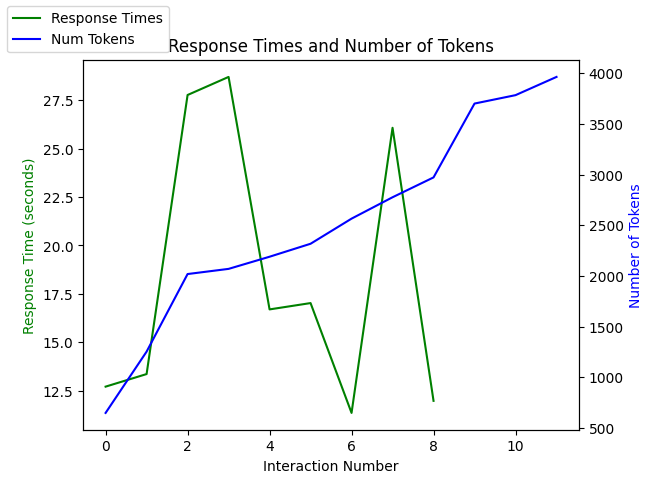
\includegraphics[width=0.7\textwidth]{images/resp-time-num-tokens.png}
    \caption{Time and number of tokens throughout the turns in a conversation.}
    \label{fig:time-tokens}
\end{figure}

Another difficulty resides in the memory--the context length--that a model can withstand. LLaMa 3.1 8B has an extremely elevated endurance, supporting a 128K context length; still, the number of tokens involved in the strategies adopted increases exponentially, making it difficult to tackle numeroues multi-turn conversation in the long run. Related to this last issue, is the time required to generate an output. Figure \ref{fig:time-tokens} shows that there is not a correlation between the number of tokens generated and the time required to give an output, though it demonstrates that it can take up to 30 seconds to produce a response, as it can significantly influence the user experience.

In conclusion, prompt engineering combined with integrating external tools significantly enhances the capabilities of language models, demonstrating that high computational resources are not strictly necessary for achieving effective, natural, and productive interactions. However, as observed through examples, this strategy is not without limitations. The model's reliance on fixed foundational weights can lead to hallucinations—plausible yet factually incorrect outputs—as demonstrated in the unrealistic recommendation of a gondola ride on Verona's Adige River, or the misinformed advice about visiting Giardini Giusti during peak sunlight hours.

Furthermore, the issue of context length and memory remains critical. Even models such as LLaMa 3.1 8B, capable of handling extended contexts of up to 128K tokens, can still face significant performance challenges due to exponentially increasing token counts in complex, multi-turn conversations. Additionally, response times, though not directly correlated with the number of tokens generated, can occasionally become prohibitively long, posing practical constraints on user experience.

Future research must focus on mitigating hallucinations, optimizing context management strategies, and improving generation speed to fully harness the potential of prompt-driven and tool-integrated language models, thus making these approaches robust, reliable, and truly beneficial for practical applications.